% ---------------------------------------------------------------------------- %
\chapter{Results}
\label{ch:results}
% ---------------------------------------------------------------------------- %
In this Section, the results obtained with the Linguometer are presented.
By the time the author is working at this Thesis, the main result accomplished
is the simultaneous acquisition of phono-articulatory features and the
consequent alignment via the \emph{LMTools2} toolkit.
It is important to clarify that out of the nine recorded experiments, three 
have been dropped due to recording problems.
Specifically, the audio mixer (\wf{AMX}) broke down during the second
experiment, thus not mixing the segmentation signals with the main speech 
signal acquired via \wf{MIC0}.
Furthermore, during the third experiment the articulograph software kept 
crashing, and it has been necessary to reboot the control computer various
times.
% ---------------------------------------------------------------------------- %
\begin{figure}[htbp]
	\centering
	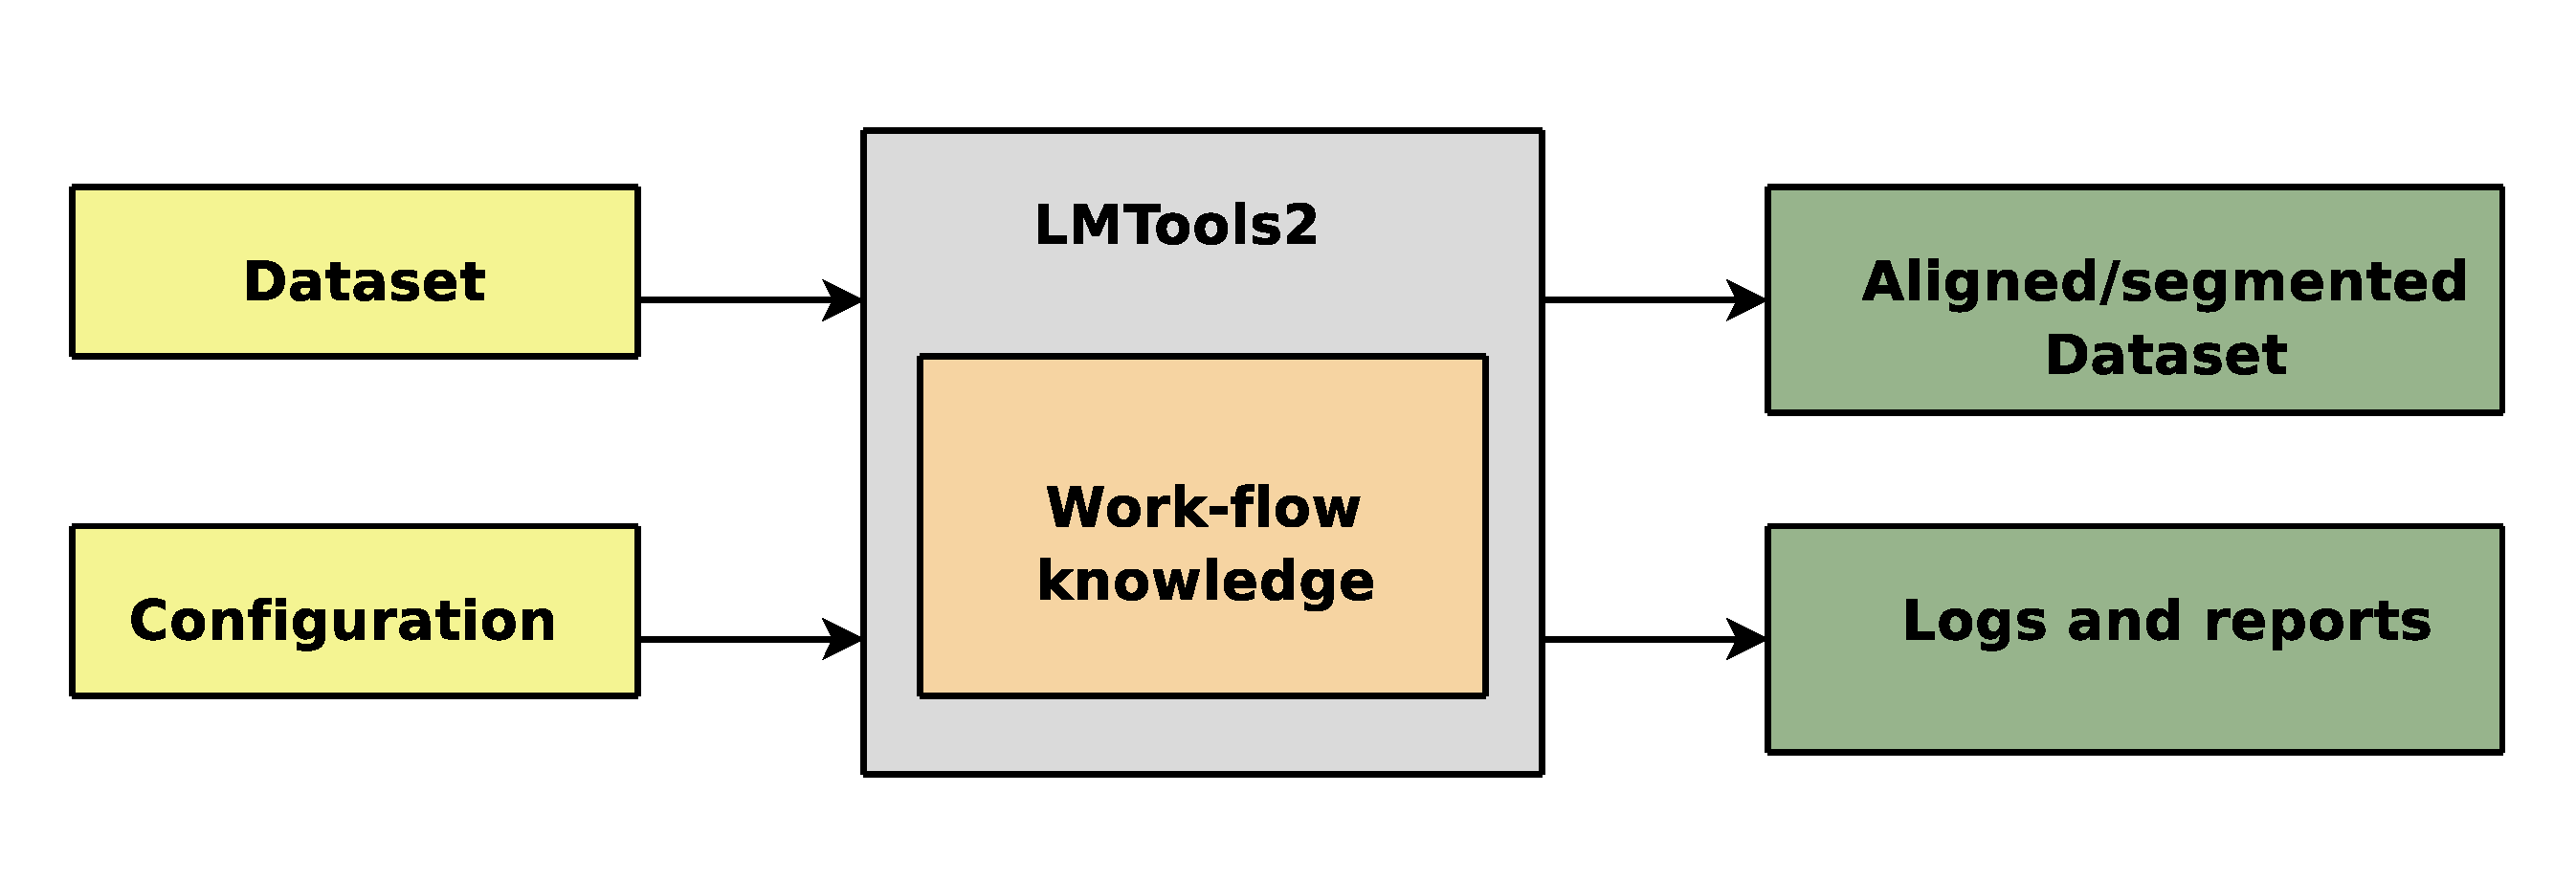
\epsfig{file=include/results/images/blackbox.eps, width=0.75\textwidth}
	\caption[LMTools2 diagram]{\textbf{LMTools2 diagram}: the \emph{LMTools2}
	toolkit operates on the dataset performing alignment and segmentation
	operations. It requires the user to compile a total of three configuration
	files, the rest of the processing is performed without the need of user
	interaction. The toolkit has been integrated using the knowledge of the
	workflow diagram, but adding new features is possible.
	The method proposed by the author produces a packaged version of the
	dataset and many informative logs and plots.}
	\label{fig:results:blackbox}
\end{figure}
% ---------------------------------------------------------------------------- %

Although those two experiments have not been recorded properly, the acquired 
data is not totally unusable.
On the other hand, the seventh experiment has been dropped since the recorded 
male subject extensively moved during the whole acquisition, often complaining
about throat pain and increased salivation.
Under those conditions the subject gets easily stressed out, performing
important head and torso movements.
As a consequence of torso movements, the articulograph frame of reference may
move, thus altering the relative position of the ultrasonograpic transducer.

As far as the author is concerned, the Linguometer integration has to be 
considered as a result by itself, and for this reason separating the
implementation from the results turns out to be a tangled task.
Moreover
the Linguometer is a personal solution provided by the author for the
problem of acquiring simultaneously a vast set of phono-articulatory
parameters.

% ---------------------------------------------------------------------------- %
%\section{Alignment and segmentation}
%\label{sec:results:alignment}
% ---------------------------------------------------------------------------- %
\subsection{Initial alignment and segmentation}
A total of nine subjects have been recorded using the Linguometer setup,
following the experimental protocol described in Section~\ref{ch:experiments}.
In Section~\ref{ch:linguometer:architecture} the workflow and the data-stream
diagrams have been presented in details.
The goal of this Section is to present the methods that allowed the author to
align and segment the acquired dataset.

It is important to underline that the data is acquired simultaneously, but the
real synchronization happens in post-processing, using a collection of tools
written by the author and called \emph{LMTools2}.
However \emph{LMTools1} and \emph{LMTools2} share the same name, they were coded
with completely different tasks in mind.
In fact, \emph{LMTools} is used to control the whole Linguometer setup, spanning
from stimuli presentation to data-acquisition and storing.
On the other hand, \emph{LMTools2} was written to automatically process large
sets of data acquired using the well determined procedure described in the
workflow diagram.

It has been said many times that the Linguometer is a constellation of hardware
and software used to acquire phono-articulatory features, and probably no better
definition exists.
The goal met by the Linguometer is the fact that a large dataset of features has
been acquired and successfully aligned.
%The novel idea behind the Linguometer 
In fact, the Linguometer setup has been integrated to meet three specifics.
Firstly, the setup has been developed to be ergonomic, since speech production
could easily be impaired if the recorded subjects distract themselves.
Furthermore, the workflow needs to be stable and flexible, in order to recover
easily from the problems that affect a small set of devices.
Lastly, the data recorded by the means of the workflow diagram does need to 
allow to batch-process the recorded data with the smallest possible degree of
human interaction.
%While the first two topics have been discussed under many aspects in
%Section~\ref{ch:linguometer} and~\ref{ch:experiments}, the latest is described
%in this Section, albeit with some degree of abstraction.\\

The \emph{LMTools2} toolkit is a collection of programs, libraries and
scripts, coded using different languages, such as C/C++, Matlab, Perl and Bash.
The C/C++ programs are used for tasks that require speed and are generally
resource-intensive, such as the detection of the synchronization and the
segmentation peaks. 
Those programs rely on a small set of optimized objects that provide an
abstract interface to data-streams and to the decoding/encoding operations.
Furthermore, particular objects are used to perform peak-detection, signal
segmentation and alignment and similar operations.
Although those programs endow some level of adaptive behavior that allow them
to recover, and eventually fix, odd behaviors, the user can easily perform
some tuning writing his own configuration files.

Generally speaking Matlab libraries and scripts are used to perform
data-analysis, plotting results and similar tasks.
Moreover, Matlab is used also to filter and align signals with an
high degree of precision, since the author found all the methods needed to
conduct similar operations.

C/C++ programs and Matlab scripts provide a consistent and uniform interface to
the data-set, albeit they perform ``atomic'' operations.
The term ``atomic'' is used since those scripts operate on small chunks of data,
such as a single sequence, a single word or even a single peak.
The atomic-level routines adaptively perform the operations they were designed
for, albeit their scope is really limited.
Similarly to what happen in operas, where the orchestra leader controls all 
the instruments, the previously described programs require to be controlled by
some program that has a larger scope on the dataset.

The task of launching the atomic-level programs is handled by a set of
\emph{LMTools2} scripts mainly written in Perl, although few of those are
written in Bash.
Being Perl a powerful and really extended language, it made the task of
automating the dataset post-processing fairly trivial.
Under normal conditions, a couple of minutes are required to write
experiment-specific configuration files, and almost 5 hours of processing 
are required to align and segment completely a single
experiment\footnote{A message for Posterity: the machine used to post-process 
the data has got an Intel Pentium D processor (SMP) running at 3.0 GHz, 2048 
MB of RAM (DDR 533 MHz) and two 10000 RPM SATA hard drive (one for reading the
RAW dataset, one for writing the alignment results). The OS of choice for
\emph{LMTools2} is Linux v2.6.20 (voluntary preemption, 200 Hz, CFQ I/O
scheduler).}.
Although the processing is really resource-intensive, the solution proposed by
the author is extremely functional.
In fact, once the configuration files have been written, the author simply
launches a script and the \emph{LMTools2} scripts handle the whole operation,
providing extended reports, plots and so on.
Figure~\ref{fig:results:blackbox} shows an exemplified \emph{LMTools2} block
diagram.
The alignment procedure can be split into two main stages: a first ``rough''
alignment and a final ``accurate'' alignment.
The need for a rough alignment stage arises from the fact that the dataset
is not recorded with a single time resolution (e.g.: 25~fps video tracks from
\wf{CC} and \wf{AG}, 200~Hz kinesthetic information from articulography data,
16~to 48~kHz audio streams).
In the final stage, where accurate alignment occurs, the data is resampled,
eventually filtered and finally aligned.

Discussing how \emph{LMTools2} work at the fine-grained level is not applicable
in the context of this Thesis since the dissertation would end up being
too long.
Many technical issues have been solved and many adaptive procedures have been
integrated into the \emph{LMTools2} toolkit\footnote{Being the \emph{LMTools2}
toolkit sources available and well documented, the author encourages the reader
to download it from: http://yarp0.cvs.sourceforge.net/yarp0/}.
Furthermore, \emph{LMTools2} is still being developed by the time the author
is writing this Thesis\footnote{The results presented in this work have been
produced with the \emph{LMTools2} updated at Jun. 21st, 2007.}.
It has been said that \emph{LMTools2} requires the user to launch a single
command in order to automatically process an experiment.
The command is GNU Make\footnote{GNU Make v3.81:
http://www.gnu.org/software/make/}, included in all Linux distribution. 
GNU Make has been designed for automatically building large application on 
Unix, and the author used it also for building the \emph{LMTools2} C/C++ code.
Moreover, Make provides a flexible and easy to use paradigm to launch
programs sequentially.

% ---------------------------------------------------------------------------- %
\subsection{Brief introduction to \emph{LMTools2}}
% ---------------------------------------------------------------------------- %
Although the author will not describe how \emph{LMTools2} works at low-level, he
decided to present the Make configuration file (Makefile) used to align and
segment each experiment\footnote{The following dissertation does not require 
any specific knowledge of GNU Make, since the method is described with some
degree of abstraction.}. 
If interested, the reader should go ahead and consult the
documentation included in \emph{LMTools2}.
The Makefile is called inside an experiment folder and the results are stored
inside dedicated folders.

\begin{scriptsize}
\begin{verbatim}
 1 CFG_NICE=config/lm_nice
 2 VAL_NICE=`if [ -e "$(CFG_NICE)" ]; then cat $(CFG_NICE); else echo 0; fi`
 3 CMD_NICE=/usr/bin/nice -n $(VAL_NICE)
\end{verbatim}
\end{scriptsize}
The first three lines are used to start the \emph{LMTools2} scripts at a given
priority. The Linux operative system (as any moder operative system does) 
privileges the execution of high-priority processes. 
In the scenario of multiprocessor systems, it is possible (ad convenient) to 
process several experiments simultaneously. 
For example, the ability to modulate priorities allows the \emph{LMTools2} 
user to decide which experiment has to be processed faster, dedicating a 
smaller amount of resources to other experiments.

\begin{scriptsize}
\begin{verbatim}
 5 all:  build process
 6 build: cleantemp prepare collect 
 7 process: cleanseq detect segment align aligncc features plot
 8 clean: cleantemp cleanseq
\end{verbatim}
\end{scriptsize}
Lines 5 to 8 define a total of four rules (e.g.: {\tt all }, {\tt clean}, 
{\tt build} and {\tt process}) using the ``{\tt rule: dependency}'' construct. 
Furthermore a dependency (e.g.: {\tt build} or {\tt detect}) is a rule by 
itself, since GNU Make will execute a set of commands to satisfy it.

\begin{scriptsize}
\begin{verbatim}
10 cleanseq:
11     echo "Cleaning seq_*/ folders"
12     $(CMD_NICE) lm_clean --noask
13
14 cleantemp:
15     echo "Cleaning temp/ folder"
16     $(CMD_NICE) lm_cleantemp --noask
\end{verbatim}
\end{scriptsize}
The {\tt echo} command simply prints its argument on the terminal, providing
useful feedback to the user. 
The  {\tt \$(CMD\_NICE)} command assigns the correct priority to the
{\tt lm\_clean} script.
In this case, {\tt lm\_clean} removes old processing results, if any is present.
Similarly, {\tt lm\_cleantemp} removes the temporary files used during
processing.

\begin{scriptsize}
\begin{verbatim}
18 prepare:	
19     echo "Preparing data for segment identification"
20     $(CMD_NICE) lm_prepare
\end{verbatim}
\end{scriptsize}
The {\tt lm\_prepare} script performs various operations, such as checking the
configuration files consistency and format conversion (e.g.: extract the audio
track from a DV stream).

\begin{scriptsize}
\begin{verbatim}
22 collect:
23     echo "Collecting data"
24     $(CMD_NICE) lm_collect
25     $(CMD_NICE) lm_exportamp
26     $(CMD_NICE) lm_exportpos
\end{verbatim}
\end{scriptsize}
The {\tt lm\_collect} script relies onto a configuration file written by the
user for collecting the necessary files from the dataset.
The files collected by the script are the output of the various devices used
during the experiments (articulograph, laryngograph, ultrasound system,
camcorder, acquisition card etc.).

\begin{scriptsize}
\begin{verbatim}
28 detect:
29     echo "Performing peak-detection"
30     $(CMD_NICE) lm_pdetect2
\end{verbatim}
\end{scriptsize}
The {\tt lm\_pdetect2} script acts as a wrapper for a C/C++ program 
(\emph{pdetect2}) that segments the \wf{CC-DV} audio tracks into the nine 
sequences an experiment is made up by.
Furthermore, it runs a peak detection algorithm onto both the \wf{US-Speech} 
and the  \wf{US-Sync}  tracks (Section\ref{ch:linguometer:architecture}).
The algorithm looks for the segmentation signals and saves the results
into a file used by other \emph{LMTools2} programs.
It may happen that the segmentation peaks are corrupted due the presence of a 
loose connection between the audio plugs, resulting in peaks that are shorter
in length and lower in amplitude, thus harder to detect.
If the peaks are still recoverable, \emph{pdetect2} recovers them. 
In the case that a single peak has been lost the program performs an estimation
of where the peak should have been.

\begin{scriptsize}
\begin{verbatim}
32 segment:
33     echo "Performing segmentation"
34     $(CMD_NICE) lm_segment
\end{verbatim}
\end{scriptsize}
Relying onto the output generated by the previous script, {\tt lm\_segment}
segments, on a per-word basis, the \wf{US-DV} stream.
The output of this script is a sequence of short DV movies, each one containing
the ultrasonograpic reconstruction of a pronounced word (a chunk of the
\wf{US-Video} track) and the corresponding speech/synchronization signals
(\wf{US-Speech} and \wf{US-Sync} respectively).

\begin{scriptsize}
\begin{verbatim}
36 align:
37     echo "Performing US<-->AG alignment"
38     $(CMD_NICE) lm_walign2
39     $(CMD_NICE) lm_splitamp
40     $(CMD_NICE) lm_splitpos
\end{verbatim}
\end{scriptsize}
The {\tt lm\_walign2} script acts a wrapper for a C++ program, \emph{walign2}.
This last program extracts the audio track from the segmented \wf{US-DV} stream,
uses the segmentation signals to align the \wf{US-Speech} track to the
\wf{AG-Speech} track and outputs the parameters needed to split the
articulograph amplitude/position data (those two operations are handled by
the {\tt lm\_splitamp} and {\tt lm\_splitpos} scripts).
While the first synchronization is done using the segmentation signals, the
second one relies onto the fact that the \wf{AG-Speech} and the \wf{AG-AMP} data
is acquired simultaneously (Section\ref{sec:linguometer:instrumentation:ag}).

\begin{scriptsize}
\begin{verbatim}
42 aligncc:
43     echo "Performing US<-->CC alignment"
44     $(CMD_NICE) lm_cleancc
45     $(CMD_NICE) lm_postcc
46     $(CMD_NICE) lm_segmentcc
\end{verbatim}
\end{scriptsize}
Once the articulograph data is aligned with the ultrasonograpic streams, the
{\tt lm\_postcc} aligns the camcorder data (\wf{CC-DV}) and the laryngographic
data with the previous two (\wf{LG-Speech} and \wf{LG-EGG}), by the means of 
cross-correlation.
The camcorder data is then segmented via {\tt lm\_segmentcc}, similarly to what
is done with the \wf{US-DV} stream.
This very last step produces a segmented, but roughly aligned version of the
original dataset.

\begin{scriptsize}
\begin{verbatim}
48 features:
49     $(CMD_NICE) lm_features
\end{verbatim}
\end{scriptsize}
The {\tt lm\_features} scripts invokes the programs needed to extract useful
features from the segmented \wf{US-DV} and \wf{CC-DV} streams.
Since those programs are still under heavy development by other CONTACT
Partners, the scripts generates a ``faked'' set of features, used by the {\tt
lm\_package} script (Line 55).

\begin{scriptsize}
\begin{verbatim}
51 plot:
52     $(CMD_NICE) lm_plotlog
\end{verbatim}
\end{scriptsize}
Before performing the final alignment on the dataset and packaging the data in
a handy format, the {\tt lm\_plotlog} script extract useful informations from
the log files and generates plots, so that the user can immediately evaluate the
quality of the alignment.

\begin{scriptsize}
\begin{verbatim}
54 pack:
55     $(CMD_NICE) lm_package
\end{verbatim}
\end{scriptsize}
Finally, the {\tt lm\_package} script handles the task of aligning, precisely,
the segmented, although roughly aligned, dataset.
The script, written in Perl, acts as a wrapper for a Matlab routine that loads,
on a per-word basis, the segmented dataset aligning it by the means of
cross-correlation.

% ---------------------------------------------------------------------------- %
\begin{figure}
  \centering
	\subfigure[\label{fig:results:uovo:aln:before}]
	{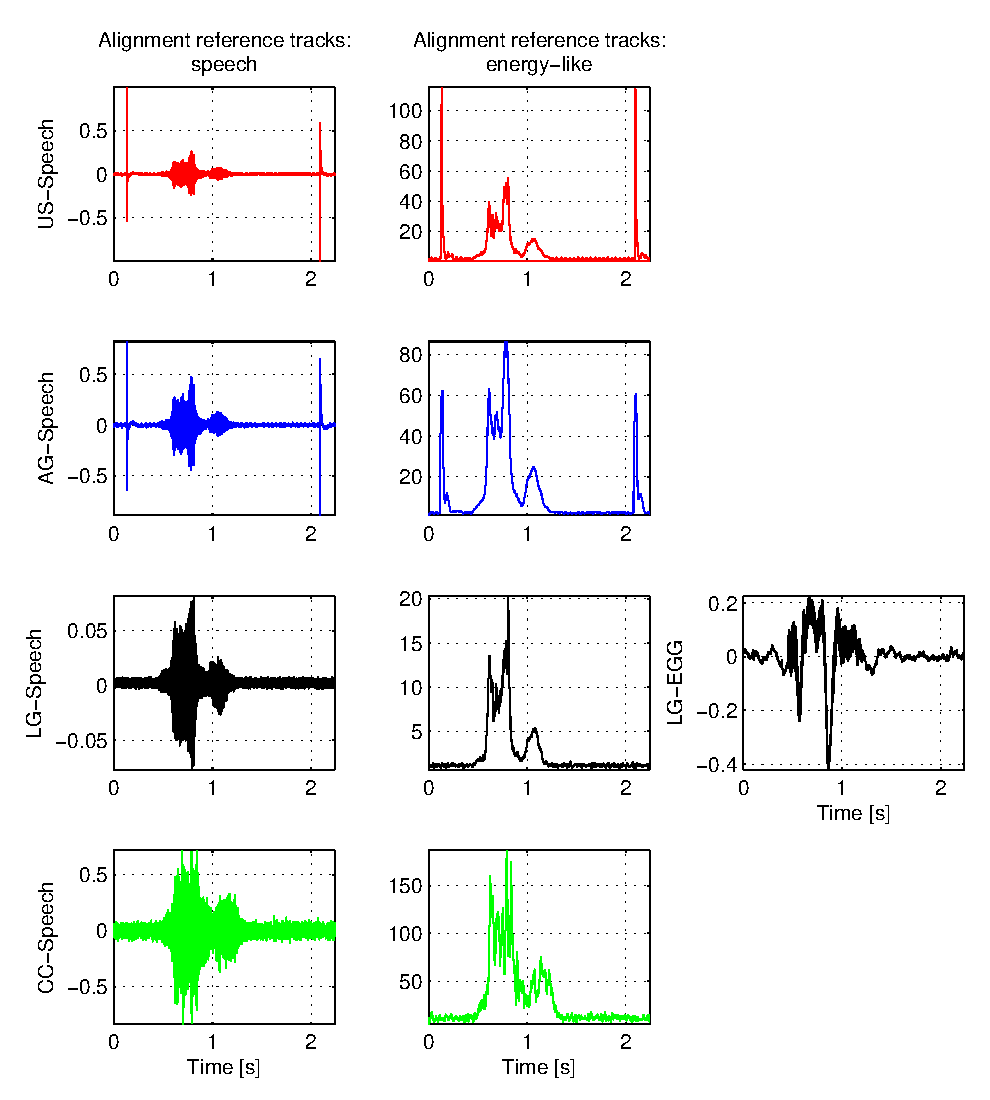
\includegraphics[width=0.45\textwidth]{include/results/images/final_15_before.eps}}
	\hspace{0.05\textwidth}
	\subfigure[\label{fig:results:uovo:aln:after}]
	{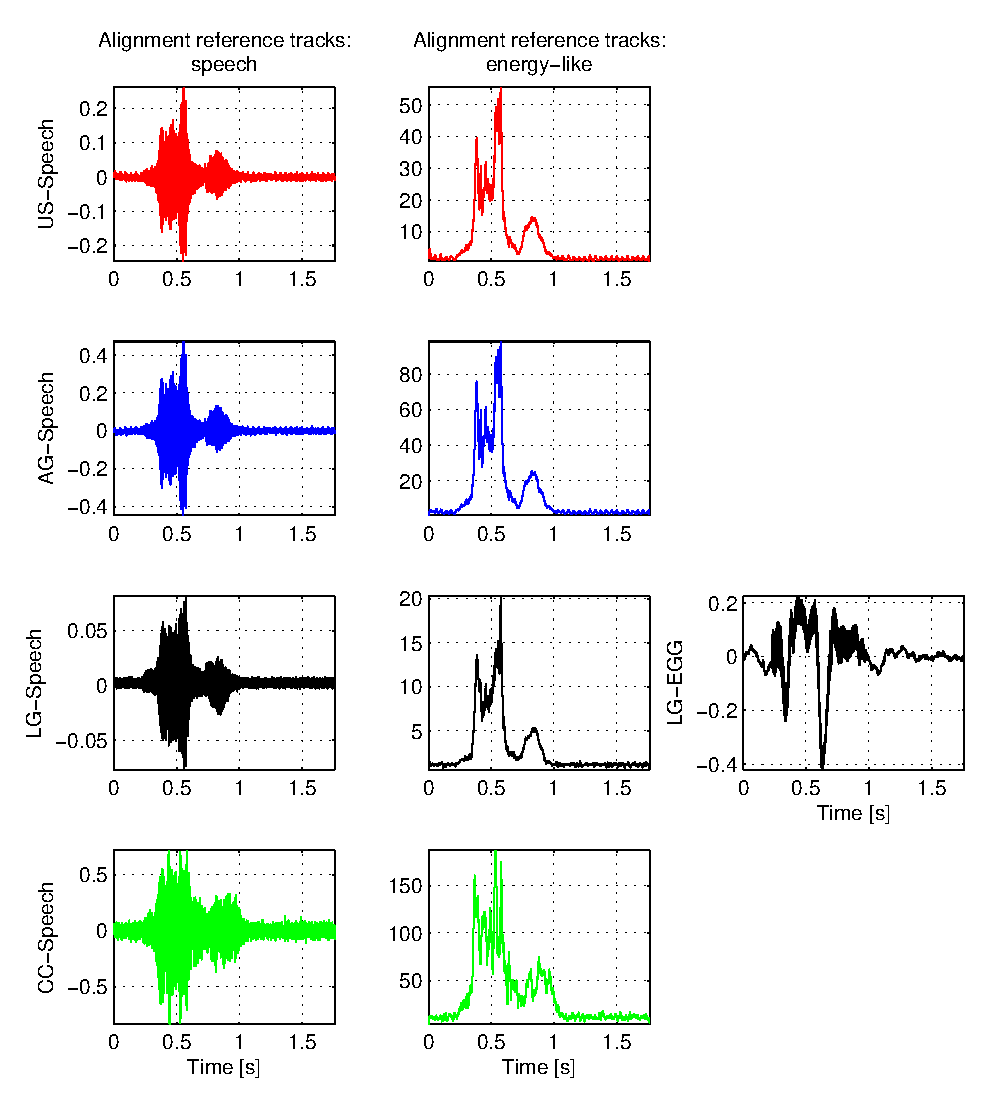
\includegraphics[width=0.45\textwidth]{include/results/images/final_15_after.eps}}

	\caption[Alignment results for /uovo/]{\textbf{Alignment
	results for /uovo/}: 
	The \wf{US-Speech} signal is used as reference during the alignment via the
	{\tt lm\_packages} Perl script.
	As P. Fitzpatrick initially suggested, the alignment is performed by
	the means of cross-correlation between ``energy-like'' signals.
	Those last signals correspond to a smoothed version of the absolute values
	of the speech signals.
	The data before alignment is shown in (a), while (b) shows the same signals
	after alignment.
	For each panel, the energy-like signals are shown. 
	Before performing the alignment procedure, the segmentation 
	peaks are removed from \wf{US-Speech} and \wf{AG-Speech}. In fact, the
	segmentation peaks visible in (a) are not visible in the final alignment 
	results (b).
	No information  about \wf{US-Video} or \wf{CC-Video} is shown, since the
	feature extraction algorithms are still under development.
	Furthermore, the \wf{AG-AMP} and the \wf{AG-POS} data are not shown in this
	Figure due their multi-dimensional nature.
	}
	\label{fig:results:uovo:aln}
\end{figure}
% ---------------------------------------------------------------------------- %

Figure~\ref{fig:linguometer:architecture:workflow} illustrates the workflow
diagram. It is important to stress out the fact that the speech signal (in this
case, \wf{Word 0} and \wf{Word 1}) is simultaneously sensed by different 
microphones. In fact,
each recording device is capable of acquiring 
the speech signal and some other data stream synchronously.
During the precise alignment procedure via {\tt lm\_package}, the
synchronization peaks are removed from the \wf{AG-Speech} and the
\wf{US-Speech} streams.
Furthermore, the data is resampled to 48 kHz, since this sampling rate is the
highest sampling rate available at the dataset level
(Section~\ref{ch:linguometer:instrumentation}).

% ---------------------------------------------------------------------------- %
\subsection{Precise alignment example}
% ---------------------------------------------------------------------------- %
As said before, it is impossible to describe the \emph{LMTools2} toolkit
extensively in this Thesis.
Due to the fact that no Linguometer exists without the final post-processing 
procedure, the author believes that the reader will find the final alignment
procedure interesting.
In this context, the data recorded during the pronunciation of the Italian words
/uovo/ and /giallo/ (English /egg/ and /yellow/ respectively) is presented.

% ---------------------------------------------------------------------------- %
\begin{figure}
  \centering
	\subfigure[\label{fig:results:giallo:aln:before}]
	{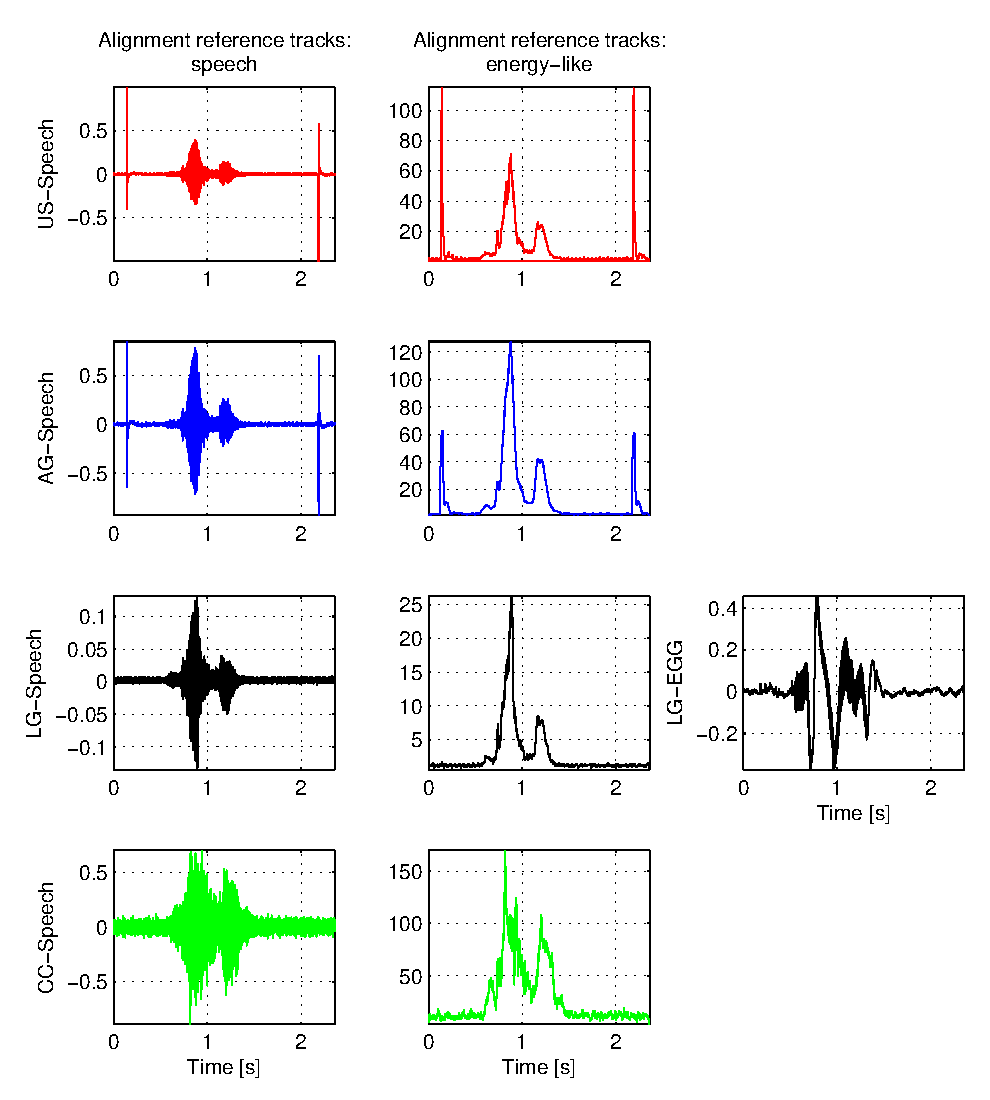
\includegraphics[width=0.45\textwidth]{include/results/images/final_20_before.eps}}
	\hspace{0.05\textwidth}
	\subfigure[\label{fig:results:giallo:aln:after}]
	{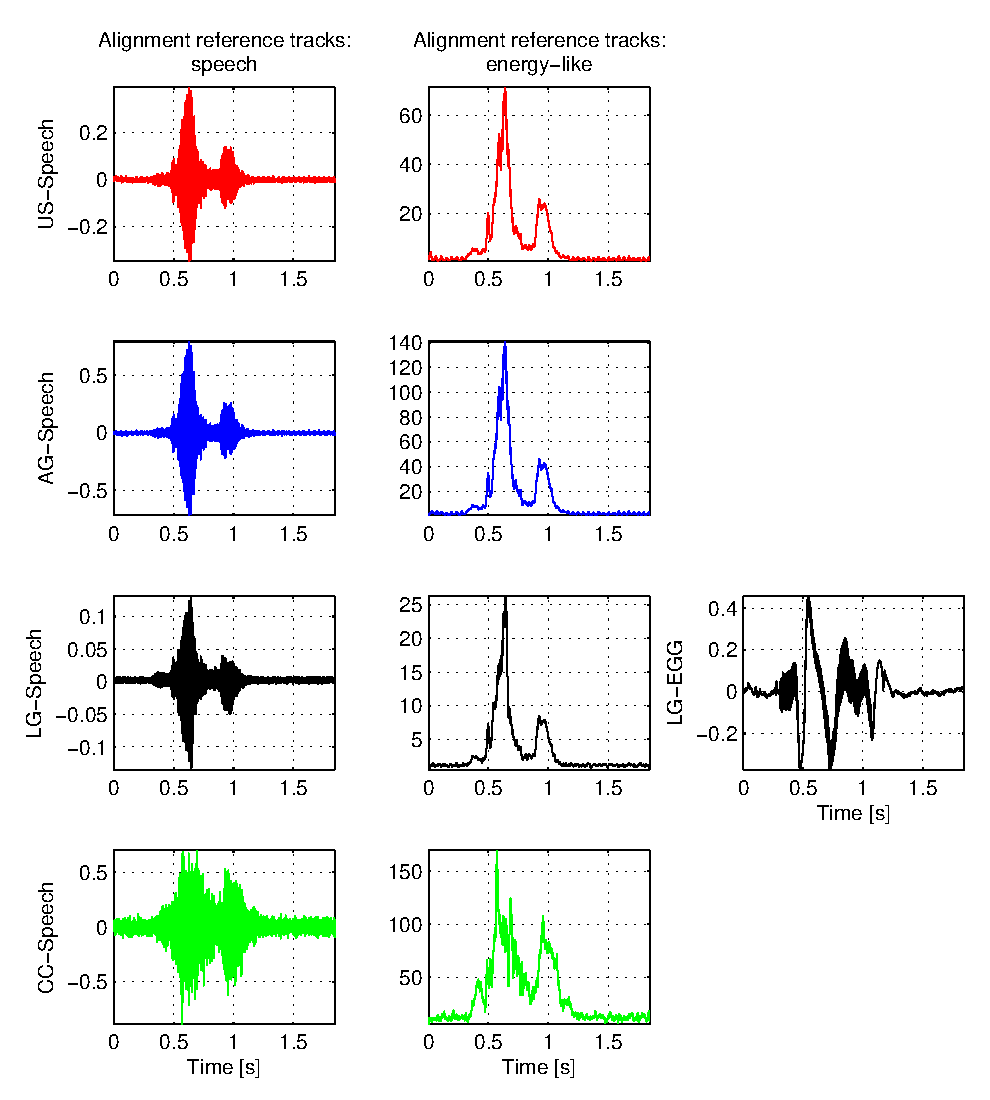
\includegraphics[width=0.45\textwidth]{include/results/images/final_20_after.eps}}

	\caption[Alignment results for /giallo/]{\textbf{Alignment results for /giallo/}: 
	data before (a) and after (b) the final alignment procedure. 
	The reader should be able to find more informative details reading the
	the caption of Figure~\ref{fig:results:giallo:aln}.}
	\label{fig:results:giallo:aln}
\end{figure}
% ---------------------------------------------------------------------------- %

It has been said that the \wf{US-DV} stream is used as reference.
Furthermore, it is assumed that the components of the \wf{CC-DV}, \wf{US-DV},
\wf{LG-WAV} and \wf{AG-DATA} streams are recorded simultaneously.
During the final alignment procedure, a Matlab routine loads the
\wf{CC-SpeechL}, the \wf{CC-SpeechR}, the \wf{LG-Speech}, the \wf{AG-Speech} 
and the \wf{US-Speech} audio signals.
The delay between each signal and the reference signal (\wf{US-Speech}) is 
calculated  applying a smoothing filter to the absolute value of the resampled
signals and then by calculating the existing lag by the means of
cross-correlation.
Once the delays are known, the appropriate correction is performed onto the
delayed or leaded signals.
Moreover, since the ``lagged'' speech signals 
(e.g.: \wf{CC-SpeechL} and \wf{CC-SpeechR}; \wf{LG-Speech}; \wf{AG-Speech})
have been recorded  simultaneously with the corresponding data signals
(e.g.: \wf{CC-Video}; \wf{LG-EEG}; \wf{AG-AMP} and \wf{AG-POS}), 
the same correction is performed on these.

It has been said that the 
{\tt lm\_features} ~script
is used to run a feature extraction algorithm both onto the \wf{CC-Video} 
and the \wf{US-Video} video streams.
By the time the author is writing this Thesis, those algorithms are under heavy
devepment, thus not available.
Two algorithms written by P. Fitzpatrick extract the profile of the moving
tongues from \wf{US-Video} and the profiles of the lips from \wf{CC-Video}.
When the time will come, it will be possible to integrate those algorithms 
inside \emph{LMTools2}, since the interfaces have been defined prior to the
development.

% ---------------------------------------------------------------------------- %
\begin{figure}
  \centering
	\subfigure[\label{fig:results:uovo:trj}]
	{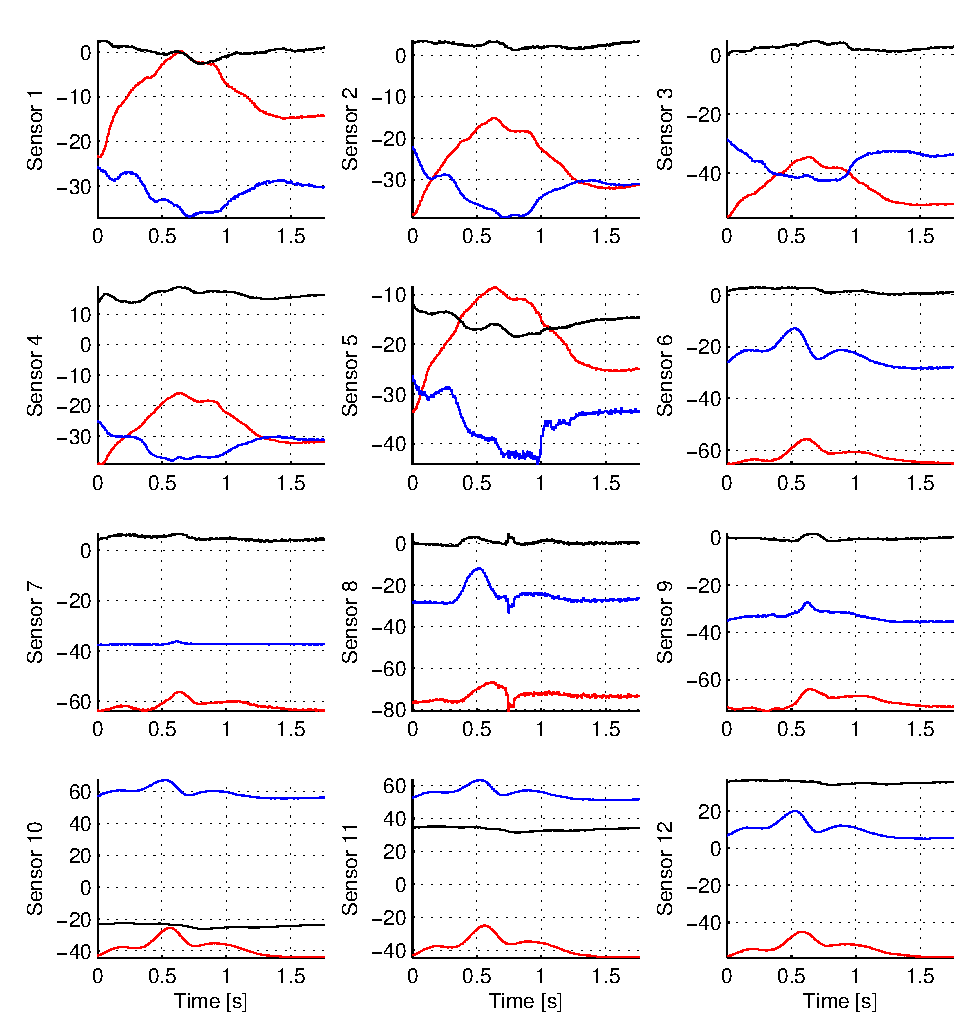
\includegraphics[width=0.45\textwidth]{include/results/images/final_15_trj.eps}}
	\hspace{0.05\textwidth}
	\subfigure[\label{fig:results:giallo:trj}]
	{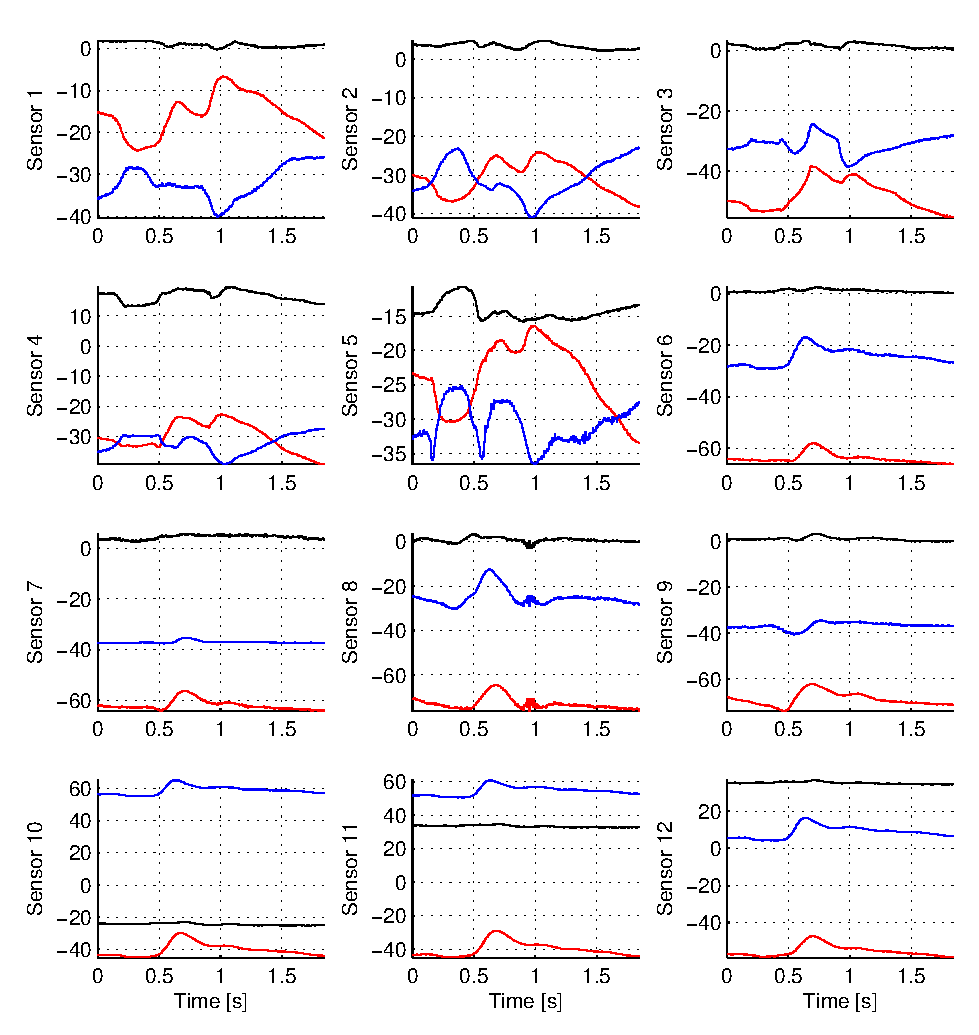
\includegraphics[width=0.45\textwidth]{include/results/images/final_20_trj.eps}}
%	\hspace{0.05\textwidth}

	\caption[Trajectories of the sensors for /uovo/ and /giallo/]{\textbf{Trajectories
	of the sensors for /uovo/ and /giallo/}: the trajectories of the twelve
	sensors during the pronunciation of the words  (a) /uovo/ and
	(b) giallo are here shown.
	The red curves represent the \emph{x} Cartesian component of the
	trajectories, while the black and the blue ones represent the \emph{y} and 
	\emph{z} coordinates.
	Note: the \emph{Phi} and \emph{Theta} angles are not shown.}
	\label{fig:results:trajectories}
\end{figure}
% ---------------------------------------------------------------------------- %
 
The main idea behind the interface between those algorithms and \emph{LMTools2}
consists in generating, on a per-word basis, a suitable data structure
(e.g.: a vector of positions) for each \wf{US-Video} and \wf{CC-Video} frame.
Temporarily, {\tt lm\_features} generates ``faked'' feature vectors,
so that it is still possible to verify the results of the alignment process.
Figures~\ref{fig:results:uovo:aln} and~\ref{fig:results:giallo:aln} show the
results of the alignment procedure for /uovo/ and /giallo/ respectively.
The \wf{AG-AMP} and the \wf{AG-POS} signals are omitted from the plots
since it is hard to represent them.
Similarly, the features extracted from \wf{US-Video} and \wf{CC-Video} are not
shown since they do not represent any physical event (e.g.: feature vectors
created randomly).
On the contrary, the \wf{LG-EGG} signal is plotted, since it is acquired by the
laryngograph as a standard audio signal. 

After the alignment has been performed, the signals are cropped so that they 
have the same length in samples. At this point the word-related data is saved to
standard Matlab ``MAT-Files'' and to custom ASCII files, thus allowing the 
processed dataset to be easily shared between the CONTACT Project partners and
in future, to the whole research community.
% ---------------------------------------------------------------------------- %
\subsection{An example of the collected data}
% ---------------------------------------------------------------------------- %
Figures~\ref{fig:results:uovo:aln} and~\ref{fig:results:giallo:aln} show the
diagnostic plots produced by \emph{LMTools2} as a support to the final
validation task.
The two figures illustrate the speech and the EGG signals before and after the
final alignment procedure. As an example, the author choose to use the /uovo/
and the /giallo/ Italian words recorded during the first experiment from a 23
years old female subject (Table~\ref{tab:experiments:subjects}).
No phonetical or motoric analysis will be presented in the context
of this dissertation, albeit the author will try to provide a good example 
of the recorded data.
The lip-tracking and the tongue-tracking algorithms are still being developed,
and for this reason few extracted frames are showed in this Section.
Furthermore, as explained in the captions of Figures~\ref{fig:results:uovo:aln}
and~\ref{fig:results:giallo:aln}, plotting the kinesthetic features acquired
using the articulograph is not trivial due to their high intrinsic 
dimensionality (Section~\ref{sec:linguometer:instrumentation:ag}).

% ---------------------------------------------------------------------------- %
\begin{figure}
  \centering
	\subfigure[\label{fig:results:uovo:complex:glasses}]
	{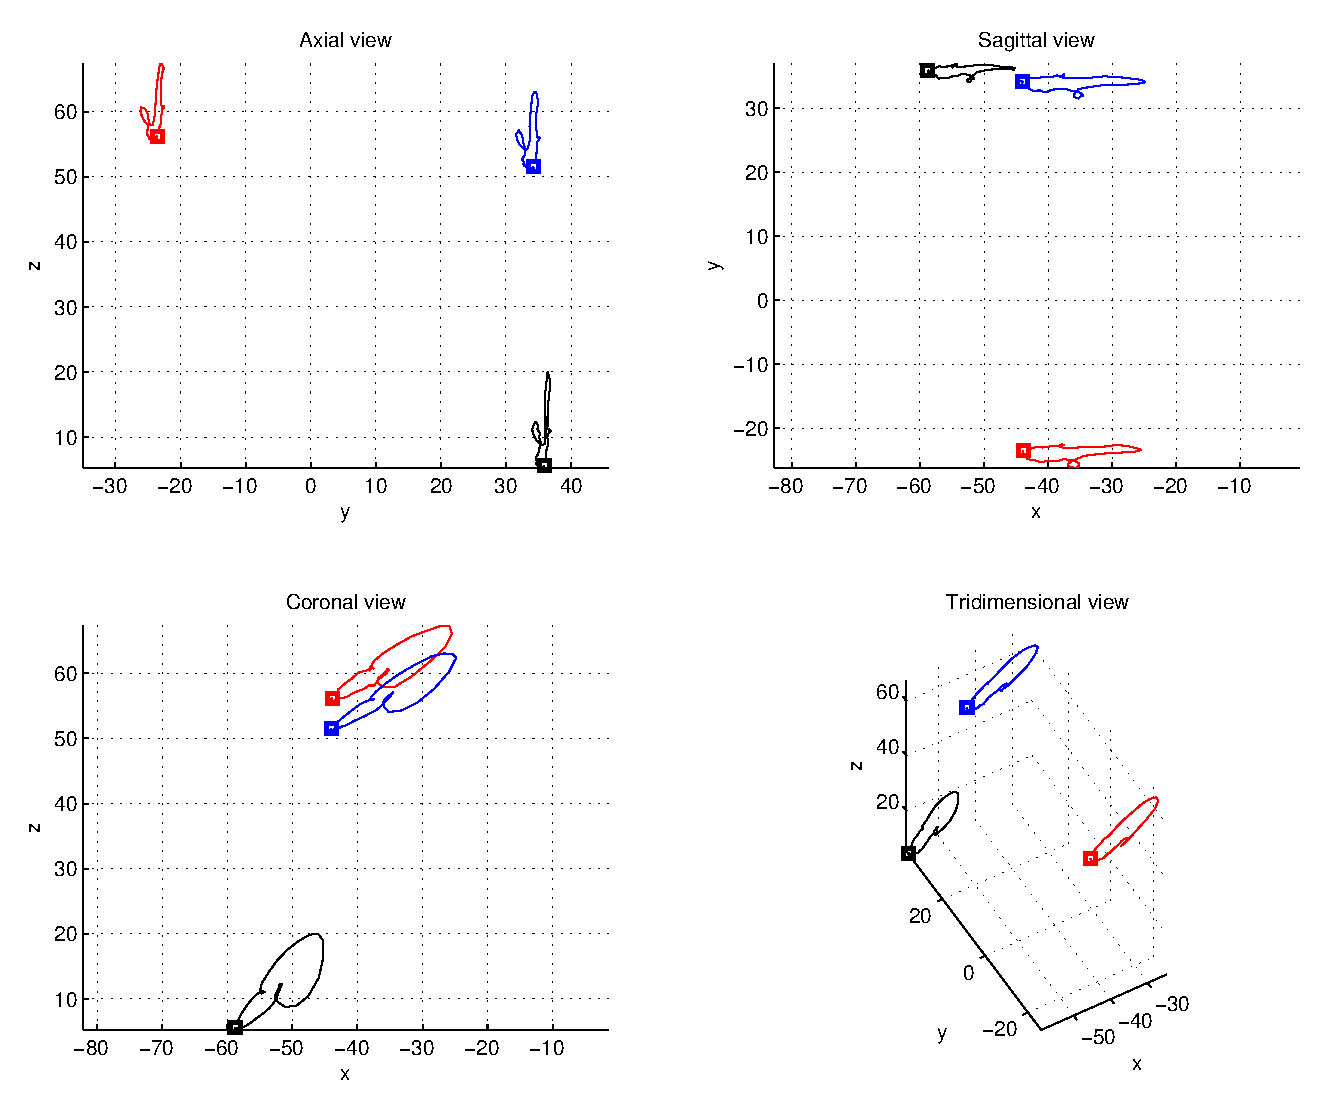
\includegraphics[width=0.45\textwidth]{include/results/images/complex_15_glasses.eps}}
	\hspace{0.05\textwidth}
	\subfigure[\label{fig:results:uovo:complex:tongue}]
	{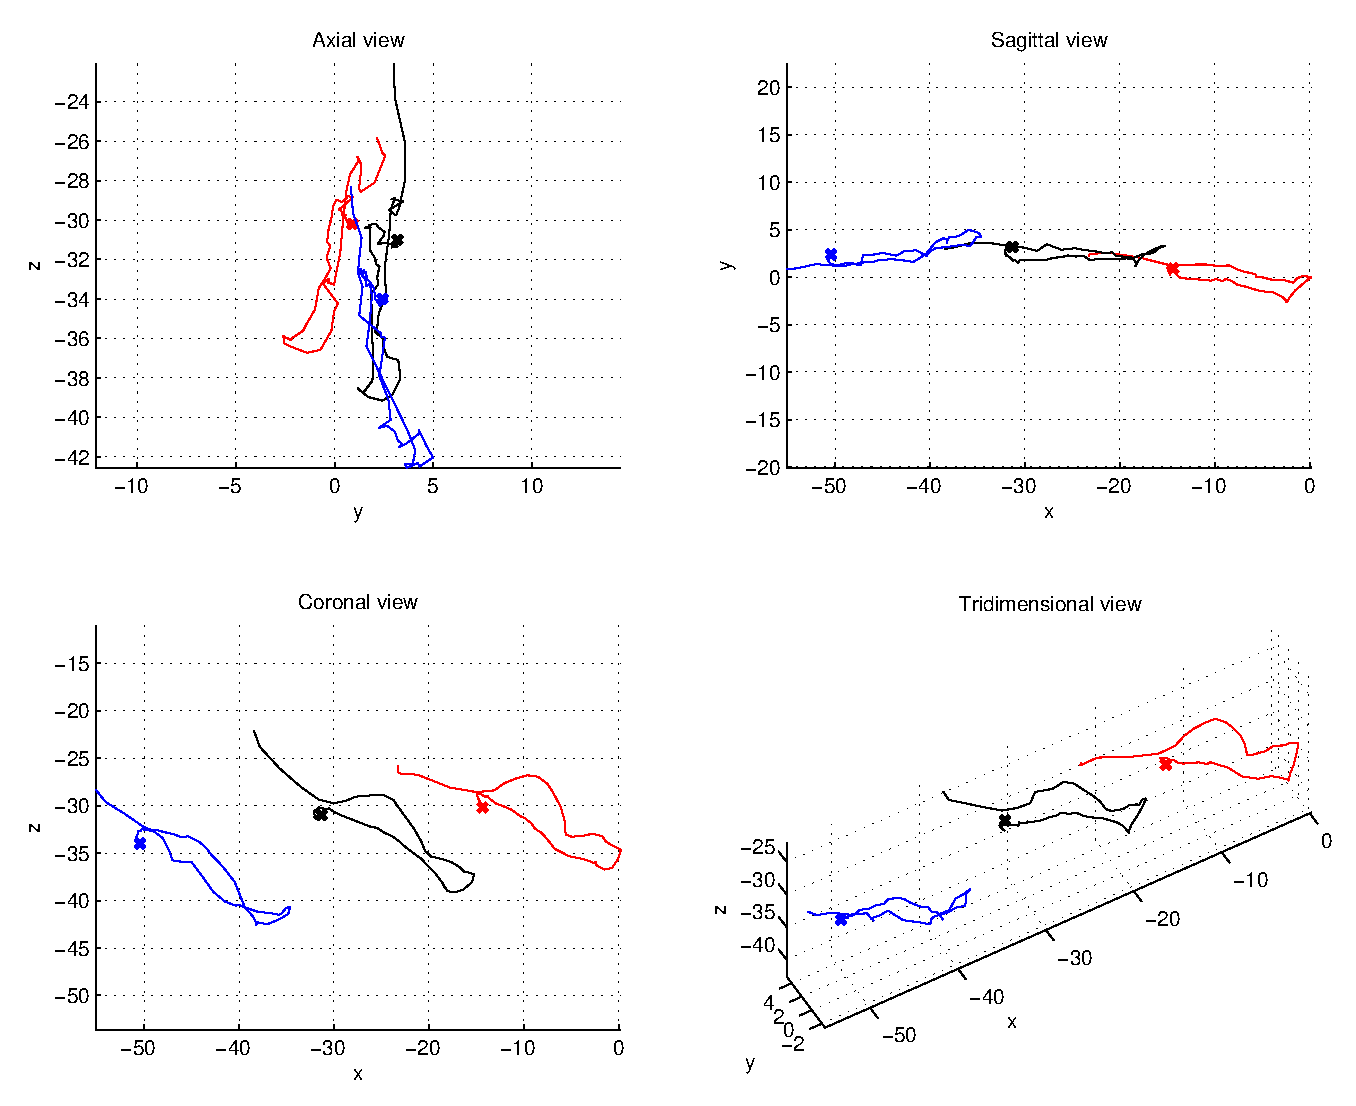
\includegraphics[width=0.45\textwidth]{include/results/images/complex_15_tongue.eps}}

	\caption[Projections of the trajectories of few sensors for 
	/uovo/]{\textbf{Projections of the trajectories of few sensors for /uovo/}: 
	a graphical representation of the trajectories of few sensors is here
	shown for the head-reference sensors (a) and for the three sensors glued 
	sagittally to the dorsum of the tongue (b).
	For each panel (a and b), the axial projection (\emph{yz} plane), 
	the sagittal
	projection (\emph{xy} plane) and the coronal projection (\emph{xz}) are
	shown.
	Furthermore, a tridimensional plot of the trajectories is provided.
	It is important to underline that the subject is looking towards the
	negative direction of the \emph{x} axis.
	Note: (a) sensor 10 in blue, sensor 11 in red and sensor 12 in black; 
	(b) sensor 1 in red, sensor 2 in black and sensor 3 in blue.
	This plot adheres to the convention shown in 
	Figure~\ref{fig:experiments:map}.
	The thick marks indicate the final position of the sensors.
	}
	\label{fig:results:uovo:complex}
\end{figure}
% ---------------------------------------------------------------------------- %

% ---------------------------------------------------------------------------- %
\begin{figure}
  \centering
	\subfigure[\label{fig:results:giallo:complex:glasses}]
	{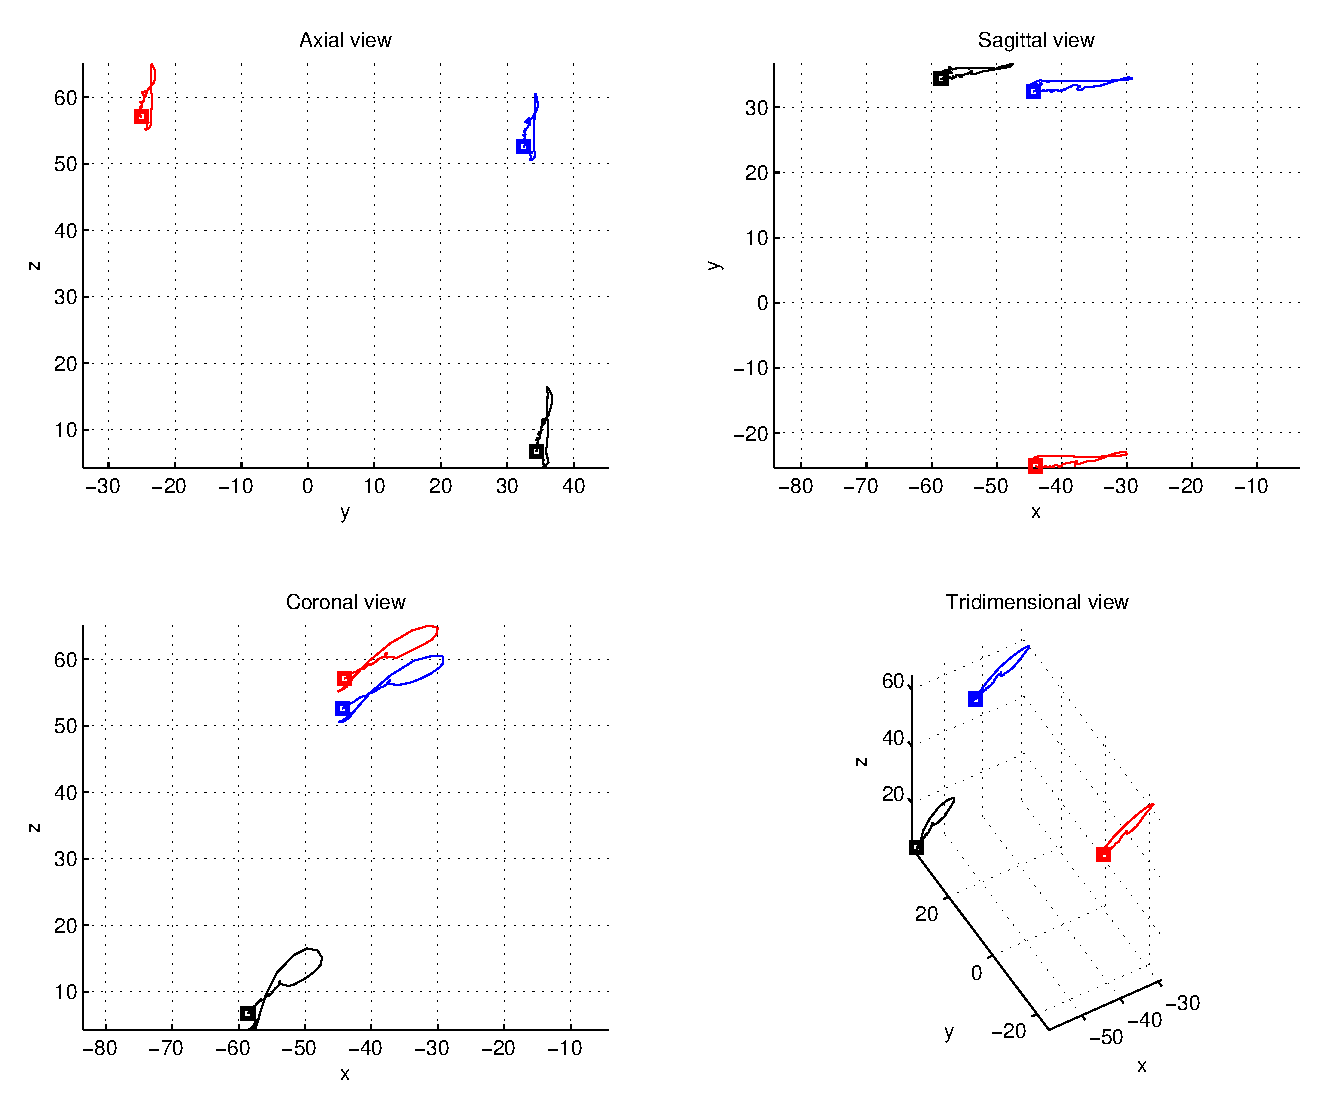
\includegraphics[width=0.45\textwidth]{include/results/images/complex_20_glasses.eps}}
	\hspace{0.05\textwidth}
	\subfigure[\label{fig:results:giallo:complex:tongue}]
	{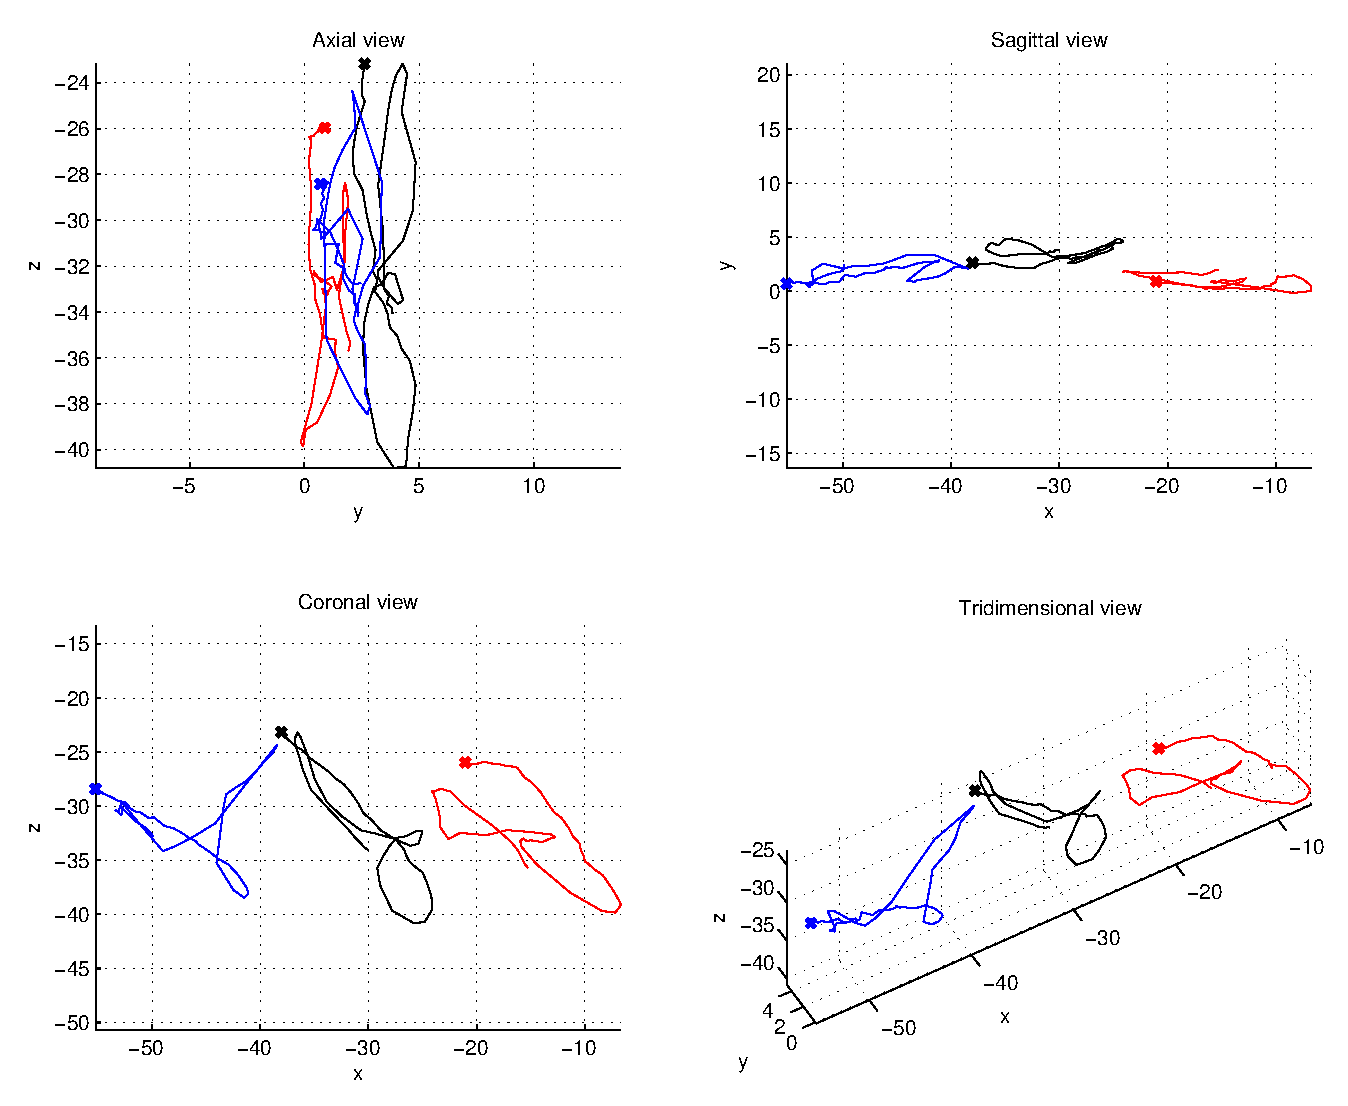
\includegraphics[width=0.45\textwidth]{include/results/images/complex_20_tongue.eps}}

	\caption[Projections of the trajectories of few sensors for /giallo/]{\textbf{Projections of the trajectories of few sensors for /giallo/}: 
	the reader should refer to the caption of
	Figure~\ref{fig:results:uovo:complex}.
	Note: (a) sensor 10 in blue, sensor 11 in red and sensor 12 in black; 
	(b) sensor 1 in red, sensor 2 in black and sensor 3 in blue.
	This plot adheres to the convention shown in 
	Figure~\ref{fig:experiments:map}.
	The thick marks indicate the final position of the sensors.
	}
	\label{fig:results:giallo:complex}
\end{figure}
% ---------------------------------------------------------------------------- %

% ---------------------------------------------------------------------------- %
\begin{figure}
  \centering
	\subfigure[\label{fig:results:mesh:complex:uovo}]
	{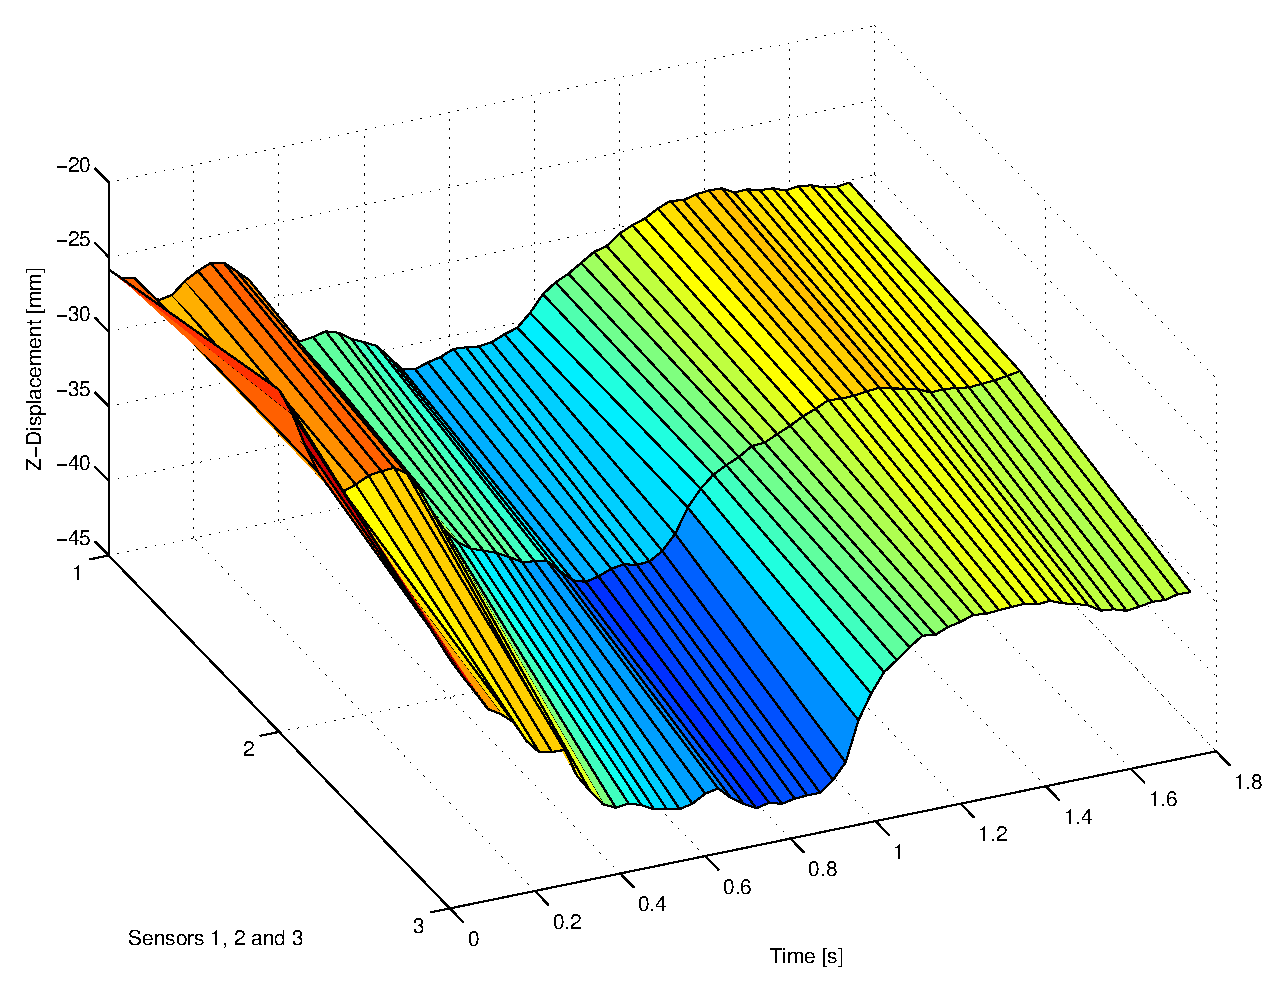
\includegraphics[width=0.45\textwidth]{include/results/images/complex_15_mesh.eps}}
	\hspace{0.05\textwidth}
	\subfigure[\label{fig:results:mesh:complex:giallo}]
	{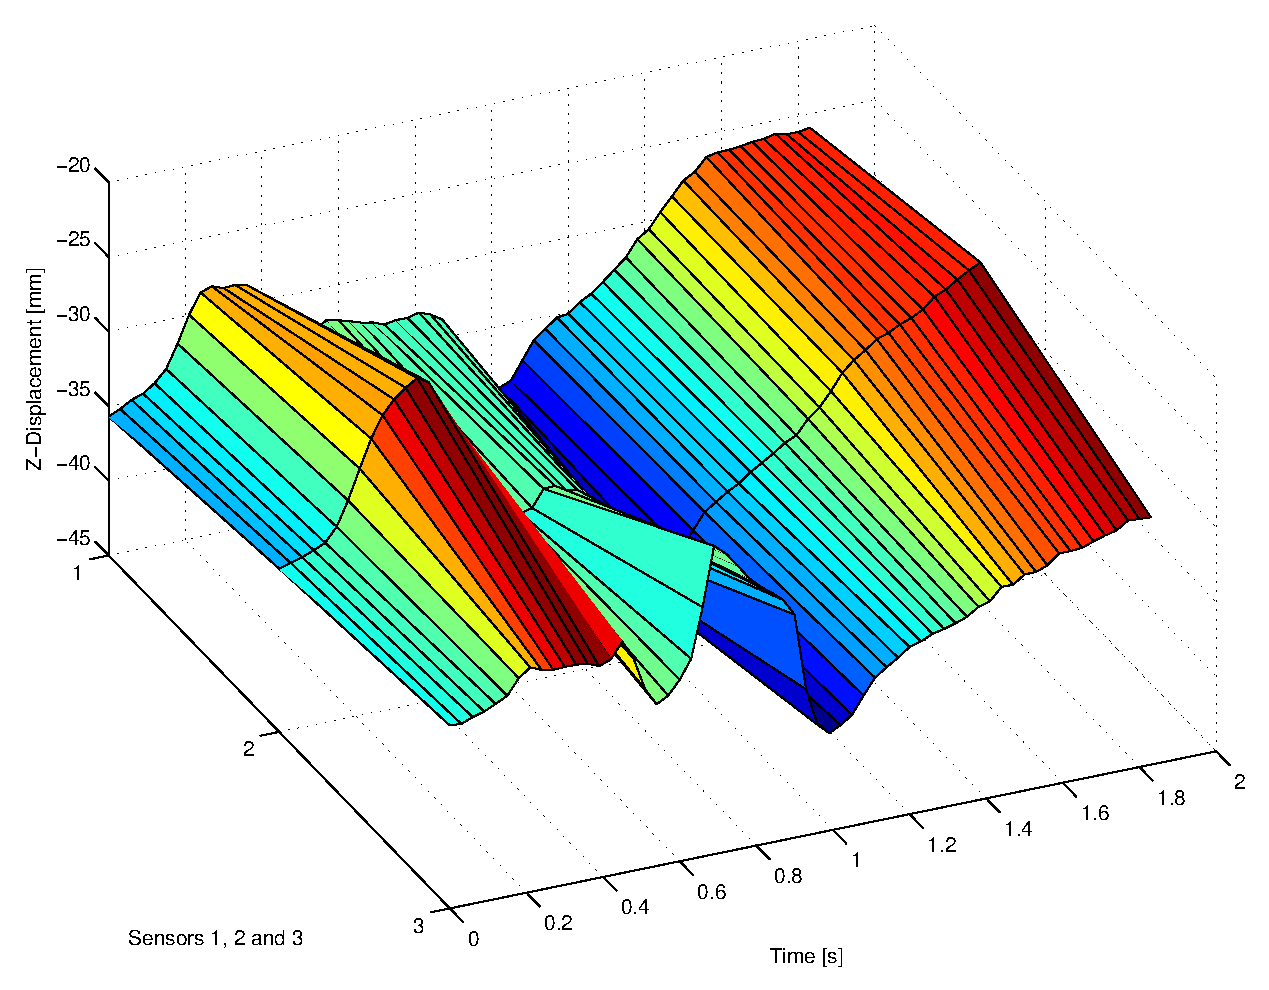
\includegraphics[width=0.45\textwidth]{include/results/images/complex_20_mesh.eps}}

	\caption[Vertical displacement of tongue for /uovo/ and /giallo/ (sagittal
	plane)]{\textbf{Vertical
	displacement of tongue for /uovo/ and /giallo/ (sagittal plane)}: 
	this plot provides a qualitative example for the vertical motion of the
	sensors glued sagittaly onto the tongue dorsum (sensors 1, 2 and 3).
	The kinesthetic information is acquired by the AG500 articulograph at
	a rate of 200 Hz. For the sake of simplicity, the data has been down-sampled
	by a factor of 6 before generating this plot (200 Hz / 6 = 33.3 Hz).
	}
	\label{fig:results:mesh:complex}
\end{figure}
% ---------------------------------------------------------------------------- %

The Cartesian coordinates of trajectories acquired from the twelve sensors 
during the pronunciation of /uovo/ and /giallo/ are shown, from a temporal
perspective, in Figure~\ref{fig:results:trajectories}.
Similarly, Figures~\ref{fig:results:uovo:complex}
and~\ref{fig:results:giallo:complex} show the projections onto the sagittal, 
the axial and the coronal plane of the sensors positioned sagittally onto the 
tongue dorsum and of the sensors taped to the glasses to track head movements.
Those last plots do not include any time information, although the
trajectories of the sensors are fully visible.
By simply looking at the Figures just mentioned, it could be said that the
pronunciation of /uovo/ recruits a more continuous movement of the tongue than
/giallo/. 
It is also clear that during the pronunciation of the submitted stimuli the head
moves, mainly due jaw motion. 
Moreover, the head reference sensors form, qualitatively, closed-loop
trajectories since the starting point and the ending point overlap. 
Figures~\ref{fig:results:mesh:complex} shows the vertical displacement of the
sensors positioned sagittally onto the tongue dorsum from a space temporal 
perspective.

% ---------------------------------------------------------------------------- %
\begin{figure}
  \centering
	\subfigure[\label{fig:results:ccs:uovo}]
	{\includegraphics[width=0.45\textwidth]{include/results/images/frames_cc_15.tps}}
	\hspace{0.05\textwidth}
	\subfigure[\label{fig:results:ccs:giallo}]
	{\includegraphics[width=0.45\textwidth]{include/results/images/frames_cc_20.tps}}

	\caption[Facial expressions during /uovo/ and /giallo/]{\textbf{Facial 
	expressions during /uovo/ and /giallo/}. 
	Also look at Figures~\ref{fig:results:uovo:cc}
	and~\ref{fig:results:giallo:cc}.}
	
	\label{fig:results:ccs}
\end{figure}
% ---------------------------------------------------------------------------- %

% ---------------------------------------------------------------------------- %
\begin{figure}
  \centering
	\subfigure[\label{fig:results:usss:uovo}]
	{\includegraphics[width=0.45\textwidth]{include/results/images/frames_us_15.tps}}
	\hspace{0.05\textwidth}
	\subfigure[\label{fig:results:uss:giallo}]
	{\includegraphics[width=0.45\textwidth]{include/results/images/frames_us_20.tps}}

	\caption[Tongue motion during /uovo/ and /giallo/]{\textbf{Tongue motion during 
	/uovo/ and /giallo/}: 21 frames extracted from the \wf{US-Video} stream are
	shown. It is important to specify that the images have been cropped.
	Furthermore, in order to enhance the quality of the printed images, a linear
	transformation has been applied so that the colors are inverted.
	Also look at Figures~\ref{fig:results:uovo:us}
	and~\ref{fig:results:giallo:us}.}
	\label{fig:results:uss}
\end{figure}
% ---------------------------------------------------------------------------- %

In order to provide an example of the data acquired using the camcorder and the
ultrasound system, the author used the seeking capabilities of the 
\emph{LMTools2} C++ library combined with the final alignment results.
The onset of speech has been initially detected in the \wf{US-Speech} main 
speech signal recorded during the pronunciation of /uovo/ and /giallo/, using
the finely aligned data packets (the speech signals used for this example are
shown in Figures~\ref{fig:results:uovo:aln} and~\ref{fig:results:giallo:aln}).
Once the onset of speech was detected onto~\wf{US-Speech} signal, the author
marked the same time instant onto the aligned \wf{CC-Speech} signal.
%A similar procedure has been followed to calculate the duration of the speech
%signals.
Once the time instants that characterize the beginning and the end of the
speech signals were known, the author sought for the corresponding video
frames both onto the \wf{US-Video} and the \wf{CC-Video} streams, thus
extracting  the video frames contained into the previously described interval.
Furthermore, since the seeking operation relies onto the final aligned data,
the extracted frames represent the same physical event, that is the
pronunciation of a word, under different perspectives, such as tongue motion and
facial expressions.
As a coincidence, the speech signals have a very similar time duration: /uovo/
lasts 0.82 seconds, while /giallo/ lasts 0.84 seconds.
Being the \wf{US-Video} and the \wf{CC-Video} video streams acquired at a rate 
of 25 frames per second, the time resolution is 40 milliseconds (e.g.: 1/25Hz =
0.04 seconds).
Since the difference in duration of /uovo/ and /giallo/ is lower than the 
resolution in time of the video streams (e.g.: 0.84 - 0.82 = 0.02), a
total of 21 video frames were extracted from both the steams.

Figure~\ref{fig:results:ccs} shows the 21
video frames extracted from the camcorder stream (\wf{CC-DV}), for both the
pronunciation of /uovo/ and /giallo/.
Similarly, Figure~\ref{fig:results:uss}
shows the 21 frames from the ultrasound system and digitized via the acquisition
card (\wf{ACD}, Section\ref{ch:linguometer:instrumentation:av}).
The representation of those video frames allow the reader to appreciate the
opening and the closure of the mouth, although it is not trivial to perceive
the head movement due the static nature of the sequence of frames.
It is important to stress the fact that during pronunciation of the submitted
stimuli, the subject moves her head over the sagittal axis, being the transducer
stand rigid. 
In this context, Figure~\ref{fig:results:ccs} turns out very useful to show 
why head compensation plays an important role in the acquisition of the 
kinesthetic information from the sensors attached on the glasses.
% ---------------------------------------------------------------------------- %
% ---------------------------------------------------------------------------- %
\begin{figure}[htbp]
	\centering
	\epsfig{file=include/results/images/frames_cc_15.tps, width=0.75\textwidth}
	\caption[Facial expressions during /uovo/]{\textbf{Facial expressions during /uovo/}.}
	\label{fig:results:uovo:cc}
\end{figure}
% ---------------------------------------------------------------------------- %

% ---------------------------------------------------------------------------- %
\begin{figure}[htbp]
	\centering
	\epsfig{file=include/results/images/frames_cc_20.tps, width=0.75\textwidth}
	\caption[Facial expressions during /giallo/]{\textbf{Facial expressions during /giallo/}
	.}
	\label{fig:results:giallo:cc}
\end{figure}
% ---------------------------------------------------------------------------- %

% ---------------------------------------------------------------------------- %
\begin{figure}[htbp]
	\centering
	\epsfig{file=include/results/images/frames_us_15.tps, width=0.75\textwidth}
	\caption[Tongue profile during /uovo/]{\textbf{Tongue profile during /uovo/}
	.}
	\label{fig:results:uovo:us}
\end{figure}
% ---------------------------------------------------------------------------- %

% ---------------------------------------------------------------------------- %
\begin{figure}[htbp]
	\centering
	\epsfig{file=include/results/images/frames_us_20.tps, width=0.75\textwidth}
	\caption[Tongue profile during /giallo/]{\textbf{Tongue profile during /giallo/}.}
	\label{fig:results:giallo:us}
\end{figure}
% ---------------------------------------------------------------------------- %

